% -----------------------------------------------
% Template for ISMIR LBD Papers
% 2021 version, based on previous ISMIR templates

% Requirements :
% * 2+n page length maximum
% * 10MB maximum file size
% * Copyright note must appear in the bottom left corner of first page
% * Clearer statement about citing own work in anonymized submission
% (see conference website for additional details)
% -----------------------------------------------

\documentclass{article}


\usepackage[T1]{fontenc} % add special characters (e.g., umlaute)
\usepackage[utf8]{inputenc} % set utf-8 as default input encoding
\usepackage{ismir,amsmath,cite,url}
\usepackage{graphicx}
\usepackage{color}

\def\lbd{}	% Flag to use correct LBD settings in the paper, please do not modify this line


\usepackage{lineno}
\linenumbers

% Title. Please use IEEE-compliant title case when specifying the title here,
% as it has implications for the copyright notice
% ------
\title{
%Transcribing multitrack music audio into lead sheets
Sheet Sage: Lead Sheets from Music Audio
}

% Note: Please do NOT use \thanks or a \footnote in any of the author markup

% Single address
% To use with only one author or several with the same address
% ---------------
%\oneauthor
% {Names should be omitted for double-blind reviewing}
% {Affiliations should be omitted for double-blind reviewing}

% Two addresses
% --------------
\twoauthors
 {Chris Donahue} {Stanford}
 {Percy Liang} {Stanford}

% Three addresses
% --------------
% \threeauthors
%   {First Author} {Affiliation1 \\ {\tt author1@ismir.edu}}
%   {Second Author} {\bf Retain these fake authors in\\\bf submission to preserve the formatting}
%   {Third Author} {Affiliation3 \\ {\tt author3@ismir.edu}}

% Four or more addresses
% OR alternative format for large number of co-authors
% ------------
%\multauthor
%{First author$^1$ \hspace{1cm} Second author$^1$ \hspace{1cm} Third author$^2$} { \bfseries{Fourth author$^3$ \hspace{1cm} Fifth author$^2$ \hspace{1cm} Sixth author$^1$}\\
%  $^1$ Department of Computer Science, University , Country\\
%$^2$ International Laboratories, City, Country\\
%$^3$  Company, Address\\
%{\tt\small CorrespondenceAuthor@ismir.edu, PossibleOtherAuthor@ismir.edu}
%}

% For the author list in the Creative Common license and PDF metadata, please enter author names. 
% Please abbreviate the first names of authors and add 'and' between the second to last and last authors.
\def\authorname{C. Donahue and P. Liang}

% Optional: To use hyperref, uncomment the following.
\usepackage[bookmarks=false,pdfauthor={\authorname},pdfsubject={\papersubject},hidelinks]{hyperref}
% Mind the bookmarks=false option; bookmarks are incompatible with ismir.sty.

\usepackage{cleveref}
\usepackage{booktabs}

\sloppy % please retain sloppy command for improved formatting

\begin{document}


\maketitle

\begin{abstract}

We present Sheet Sage, 
a system designed to transcribe Western multitrack music into lead sheets: human-readable scores which indicate melody and harmony. 
%\footnote{For music with vocals, lead sheets usually also include lyrics. Here we focus just on transcribing the melody and harmony.} 
The potential use cases for reliable lead sheet transcription are broad and include 
music performance, 
education, 
interaction, 
informatics, 
and generation. 
However, the task is challenging because it involves many subtasks: 
beat tracking, 
key detection, 
chord recognition,
and melody transcription. 
A major obstacle is melody transcription which, 
while arguably simpler for humans than chord recognition, 
remains a challenging task for MIR. 
Here we leverage recent advancements in audio pre-training to break new ground on this task, 
resulting in a system which can reliably detect and transcribe the melody in multitrack recordings. 
By combining this new melody transcription approach with existing strategies for other subtasks, 
Sheet Sage can transcribe recordings into score representations which echo the musical understanding of human experts.\footnote{Examples: \url{http://chrisdonahue.com/sheetsage-lbd}}
\end{abstract}

\section{Introduction}\label{sec:introduction}

\begin{figure*}
    \centering
    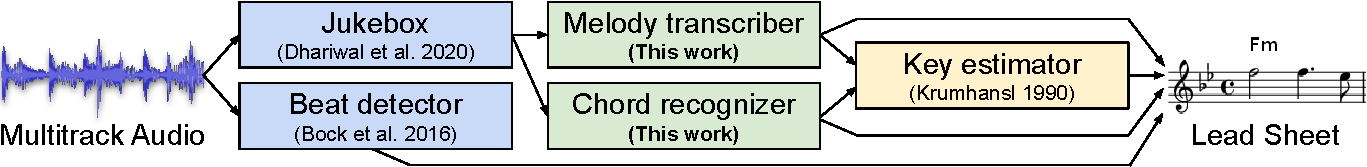
\includegraphics[width=\linewidth]{figs/one.pdf}
    \caption{Inference procedure for Sheet Sage, our proposed system which transcribes multitrack audio into lead sheets (scores which depict melody as notes and harmony as chord names). The blue, green, and yellow boxes respectively take audio, features, and symbolic music data as input. Green boxes are modules that we built as part of this work---both are Transformers~\cite{vaswani2017attention} trained on their respective tasks using audio features from Jukebox~\cite{dhariwal2020jukebox} and data from Hooktheory~\cite{hooktheory}.}
    \label{fig:one}
\end{figure*}

In the Western music canon, 
a musical composition can often be characterized by its melody and harmony. 
% This information can be depicted on a lead sheet---a musical score which contains the melody as notes on a staff and the harmony as chord names. 
% When interpreted by a musician, 
% a lead sheet can be used to perform recognizable renditions of existing pieces.
When engraved as a \emph{lead sheet}---a musical score containing the melody as notes on a staff and the harmony as chord names---melody and harmony can be readily interpreted by musicians, enabling recognizable performances of existing pieces. 
Hence, for some music, a lead sheet represents the essence of its underlying composition.

A system which reliably transcribes multitrack recordings into lead sheets could potentially enrich human music practice by
decreasing the effort required for performing existing pieces, 
which in turn might also increase engagement in music education through curricula tailored to student preferences. 
Moreover, such a system could act as a preprocessing component for MIR pipelines to help facilitate 
interaction~\cite{},
informatics~\cite{bainbridge1999towards}, 
retrieval~\cite{}, 
source separation~\cite{ewert2014score}, 
and generation~\cite{hawthorne2019enabling}. 
Despite the numerous potential benefits, 
to the best of our knowledge such a system does not currently exist, 
and building one is challenging as it amounts to the amalgamation of many difficult MIR tasks: 
beat tracking, 
key detection, 
chord recognition, 
and melody transcription.

Among these tasks, 
\emph{melody transcription}---defined here as converting multitrack audio to a time-aligned, monophonic sequence of equal-tempered notes constituting its melody---is arguably the furthest from a reliable solution. 
A closely-related problem that has received considerable attention in MIR is \emph{melody extraction}~\cite{goto2000robust}, 
which involves estimating the time-varying fundamental frequency trajectory of the melody in multitrack audio (see~\cite{salamon2014melody} for a comprehensive review). 
While melody extraction is useful for several downstream tasks and is more inclusive of music which does not use equal temperament, 
its outputs cannot be readily converted into familiar music formats like MIDI or scores. 
It is possible to segment the outputs of melody extraction into notes~\cite{nishikimi2016musical}, 
however it stands to reason that directly transcribing audio could sidestep the pitfalls of pipeline-based approaches. 
% While melody transcription is possible by segmenting the outputs of melody extraction into notes~\cite{nishikimi2016musical}, 
% it stands to reason that transcribing the melody from audio could outperform pipeline-based approaches.

In this work, we break new ground on melody transcription by combining advancements in audio pre-training with a large collection of labeled data for this task. 
Specifically, we collect and align around $50$ hours of paired audio segments and human-transcribed melodies from Hooktheory~\cite{hooktheory}. 
To model this dataset effectively, 
we leverage audio representations from Jukebox~\cite{dhariwal2020jukebox}, 
a generative model pre-trained on one million multitrack recordings. 
These representations were recently shown to be powerful features for several MIR tasks~\cite{castellon2021calm}, 
and here we demonstrate that they are also useful for the task of melody transcription---a Transformer~\cite{vaswani2017attention} trained on top of these audio representations achieves
% 0.743 vs. 0.587
$27\%$ 
better performance on melody transcription 
than the same architecture trained on traditional spectrogram features.

To complete \emph{Sheet Sage}, 
our lead sheet transcription system, 
we additionally train a chord recognition model using Jukebox representations and the Hooktheory dataset.
Together, these two models give us estimated timestamps for melody note onsets and chord changes, i.e., a MIDI-like representation. 
Rendering this information as a lead sheet requires additional information: key signature and metrical structure. 
We estimate the former using the Krumhansl-Schmuckler algorithm~\cite{krumhansl1990cognitive,temperley1999key}, which takes the estimated melody and chord information as input. 
For the latter, we use \texttt{madmom}~\cite{bock2016madmom,bock2016joint} to estimate timestamps of beats and downbeats, 
which we then use to quantize the estimated melody and chord transcription to the nearest sixteenth note. 
Finally, we engrave a lead sheet using Lilypond~\cite{nienhuys2003lilypond}. 
See~\Cref{fig:one} for an overview of our system.

\section{Melody Transcription Evaluation}

\newcommand{\tabquantrow}[7]{ #7 & #1 & #2 & #3 \\}

\begin{table}[t]
\centering
\begin{tabular}{l @{\hspace{1.25\tabcolsep}} c @{\hspace{1.25\tabcolsep}} c @{\hspace{1.25\tabcolsep}} c}
\toprule
Approach & $F_1$ & $P$ & $R$ \\
\midrule

% mel 0.28663762224714356 0.28386365399857477 0.2894663409916158 0.40869955139013564 0.3939042752379466 0.424649641577061
\tabquantrow{$28.7$}{$28.4$}{$28.9$}{$40.9$}{$39.4$}{$42.5$}{Melody extraction~\cite{salamon2012melody} + Seg.}

% spt 0.37615494578146064 0.4339886306130625 0.33192265721093334 0.5576884462034533 0.5552788485277123 0.5601190476190476
\tabquantrow{$37.6$}{$43.4$}{$33.2$}{$55.8$}{$55.5$}{$56.0$}{Vocal iso.~\cite{hennequin2020spleeter} + Transcribe~\cite{mauch2015computer}}

% spta 0.46801472954538414 0.47712661516151783 0.45924434901101074 0.5576884462034533 0.5552788485277123 0.5601190476190476
\tabquantrow{$46.8$}{$47.7$}{$45.9$}{$55.8$}{$55.5$}{$56.0$}{~~~~Allow abstain for non-vocal}

% ryy 0.4867368763278077 0.47900457777551503 0.49472290693071175 0.5949184396528961 0.5823602484472049 0.608030185077476
\tabquantrow{$48.7$}{$47.9$}{$49.5$}{$59.5$}{$58.2$}{$60.8$}{Features + HMM~\cite{ryynanen2008automatic}}

% ssh 0.6004892742711208 0.6347876689011206 0.5697072579915735 0.6844009173691797 0.6886709527441793 0.6801835075493612
\tabquantrow{$60.0$}{$63.5$}{$57.0$}{$68.4$}{$68.9$}{$68.0$}{Spectro.~\cite{hawthorne2018onsets} + Transformer~\cite{vaswani2017attention}}

% ssj 0.7496230224947461 0.74844514579763 0.7508046124376337 0.863281835547652 0.8343902092739303 0.8942460317460318
\tabquantrow{$\mathbf{75.0}$}{$\mathbf{74.8}$}{$\mathbf{75.1}$}{$\mathbf{86.3}$}{$\mathbf{83.4}$}{$\mathbf{89.4}$}{Jukebox~\cite{dhariwal2020jukebox} + Transformer~\cite{vaswani2017attention}}

\bottomrule
\end{tabular}
\caption{Macro-averaged performance of different approaches for melody note onset transcription.}
\label{tab:quantitative}
\end{table}

Services like Chordify~\cite{de2014chordify} already demonstrate that it is possible to estimate all of the information needed for engraving lead sheets besides melody. 
Hence, we focus on melody transcription for our evaluation of Sheet Sage. 
To the best of our knowledge, 
Paiva~et~al.~\cite{paiva2005detection} were the first to investigate melody transcription (as opposed to extraction). 
The earliest work for which we could find code or audio examples was that of Ryyn{\"a}nen and Klapuri~\cite{ryynanen2008automatic}, 
which provides example transcriptions from their HMM-based system for $10$ segments from the RWC Music Database~\cite{goto2002rwc}. 
To facilitate direct comparison, 
we base our quantitative evaluation on this small dataset. 

\textbf{Metrics.} In our melody transcription setting where we care primarily about human readability, 
we posit that correctly identifying note onsets, 

Among metrics traditionally used to evaluate piano transcription, Ycart et al.~\cite{ycart2020investigating} demonstrate that onset-only note-level $F_1$ correlates most strongly with human judgements. 

\begin{figure}[t]
    \centering
    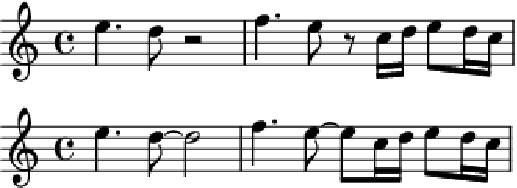
\includegraphics[width=0.95\linewidth]{figs/heuristic_offsets.pdf}
    \caption{Engraving a melody with ground truth~(top) vs. heuristic~(bottom) note offsets. Compared to predicting onsets, we argue that predicting offsets is of secondary importance for human-readable melody transcription.}
    \label{fig:heuristic_offsets}
\end{figure}

For our lead sheet setting, 
we argue that onsets are far m

See our examples page$^1$ for 

% Assumptions regarding metrics:
% For melody scores, note onset is most important
% Offsets do not dramatically improve readability
% Octave does not matter

% Observations
% Sometimes transcribes an instrument that humans do not
% Can switch between instruments

% Error analysis:
% Doubled notes
% Blows up on poor intonation

% Drawbacks
% Only 3/4 and 4/4


\section{Acknowledgements}

% John Thickstun (for conversations / mido)
% John Hewitt (for conversations)
% Nelson Liu (for tech support)
% Megha Srivastava (for feedback)
% Jen Hsu (for feedback)
% Annie (for beaming)

% For bibtex users:
\bibliography{main}

\end{document}

